\subsection{\cite{benoptical}}

An interesting component of the work by Ben-Dayan and Giloh was their experiments with stem, note head and symbol detection during the segmentation phases.

\subsubsection{Stem Detection}

For stem detection, since handwritten stems are unlikely to be perfectly straight, the authors use vertical projections combined with a high pass filter to establish likely stems. These are represented by peaks in the vertical projection.

A bounding box is then generated and the note is split into an upper and lower region; the upper and lower parts being used in note head and beam detection later.

\subsubsection{Note Head and Features Detection}

The author extracts the head position by way of a distances transform and then examining the density of the pixels (distance from the nearest black pixel) the results of which you can see graphically in \cref{fig:giloh-component-centre}. The authors also make several assumptions at this stage regarding the size of features (e.g. sharps are less than twice the stave space height) which enables them to separate notes from other components (clefs, accidentals etc).

\begin{figure}[H]
  \centering
  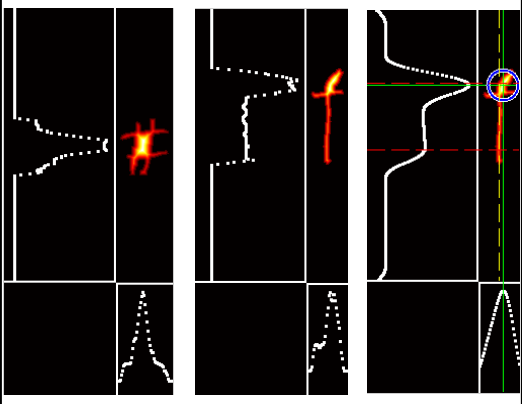
\includegraphics{gfx/prior-research/giloh-component-centre}
  \caption{Finding component centres, \parencite{benoptical}}
  \label{fig:giloh-component-centre}
\end{figure}
